%
% waermeleitung.tex -- Beispiel für Problemlösung mit finiten Differenzen
%
% (c) 2020 Prof Dr Andreas Müller, Hochschule Rapperswio
%
\subsection{Wärmeleitungsgleichung
\label{buch:subsection:waermeleitung}}
Als etwas ausführlicheres Beispiel soll in den folgenden Abschnitten
das Wärmeleitungsproblem auf einem Stab mit verschiedenen Randbedingungen
und Methoden zu lösen.
Dieser Abschnitt beginnt damit, das Problem und seine Diskretisierung
zu formulieren.
In den folgenden Abschnitten werden die Gleichungen dann für verschiedene
Randbedingungen numerisch gelöst.

\subsubsection{Die Wärmeleitungsgleichung}
Die Temperaturverteilung $u(x,t)$ auf einem Stab mit $x$-Koordinaten
zwischen $0$ und $1$ zur Zeit $t$ wird durch eine partielle
Differentialgleichung auf dem Gebiet
\[
\Omega = \{ (x,t)\;|\; 0 < x < 1\wedge 0<t\}
\]
beschrieben.
In der Wärmeleitungsgleichung
\begin{equation}
\frac{\partial u}{\partial t}
=
\kappa\frac{\partial^2 u}{\partial x^2}
\label{buch:pde:waerme:gleichung}
\end{equation}
ist die $\kappa$ eine Konstante, die Wärmeleitfähigkeit und
Wärmekapazität des Materials charaktersiert.

\subsubsection{Randbedingungen}
Zudem müssen Randbedingungen zur Zeit $t=0$ und an den Enden
des Stabes bei $x=0$ oder $x=1$ erfüllt sein.
Zur Zeit $t=0$ muss die initiale Temperaturverteilung $f(x)$ 
spezifiziert werden.

Dirichletrandbedingungen
\[
\begin{aligned}
u(x,0)&=f(x)&&x\in[0,1]
\\
u(x,t)=\frac{\partial u}{\partial x}(x,t)&=g(x)&&x\in \{0,1\}.
\end{aligned}
\]
am Rand des Intervals bedeuten, dass die Enden des Stabes mit Wärmereservoirs
verbunden sind, welche ihn auf einer vorgegebenen Temperatur halten.

Neumann-Randbedingungen
\[
\begin{aligned}
u(x,0)&=f(x)&&x\in[0,1]
\\
\frac{\partial u}{\partial n}(x,t)=\frac{\partial u}{\partial x}(x,t)&=g(x)&&x\in \{0,1\}.
\end{aligned}
\]
spezifizieren den Temperaturgradienten am Rande und legen damit fest,
wieviel Wärmeenergie in den Stab hineinfliesst oder ihn verlässt.
Im Falle $g(x)=0$ verschwindet der Gradient und Wärmefluss ist unterbunden.
Dies entspricht einem thermisch isolierten Stab.

\subsubsection{Energie}
Die physikalische Interpretation der
Gleichung~\ref{buch:pde:waerme:gleichung}
erlaubt, das Verhalten der Lösung abzuschätzen.
Dazu berechnen wir die Gesamtenergie
\[
U(t) = \int_0^1 u(x,t)\,dx,
\]
die im Intervall enthalten ist.
Die Wärmeleitungsgleichung~\ref{buch:pde:waerme:gleichung} erlaubt nun,
die Änderung der Energie mit der Zeit zu bestimmen.
Es gilt
\begin{align*}
\frac{dU(t)}{dt}
&=
\frac{d}{dt} \int_0^1 u(x,t)\,dx
=
\int_0^1 \frac{\partial u}{\partial t} (x,t)\,dx
=
\kappa \int_0^1 \frac{\partial^2u}{\partial x^2}(x,t)\,dx
=
\kappa \biggl[\frac{\partial u}{\partial x}\biggr]_0^1.
\end{align*}
Daraus lässt sich zum Beispiel ablesen, dass sich die Energie in
einem isolierten Stab, wo die Ableitungen an den Intervallenden
verschwinden, nicht ändert.
Oder dass Energie genau dann konstant bleibt, wenn die Steigung
in beiden Enden gleich gross ist, was gleichbedeutend ist damit,
dass der Wärmefluss durch beide Intervallenden gleich gross ist.

In allen Fällen kann man das Verhalten der Lösung für $t\to\infty$
bestimmen.
Dirichlet-Randbedingungen 
\[
u(0,t) = u_0 \qquad\text{und}\qquad u(1,t) = u_1
\]
sagen zum Beispiel, dass die beiden Enden des Stabes auf Temperatur
$u_0$ und $u_1$ gehalten werden.
Mit der Zeit wird sich eine stationäre Temperaturverteilung, also eine
Temperaturverteilung, die sich mit der Zeit nicht mehr ändert.
Eine solche hat zweite Ableitung
\[
\frac{\partial^2u}{\partial x^2}
=
\frac{1}{\kappa} \frac{\partial u}{\partial t} = 0.
\]
Die Funktion $x\mapsto u(x,t)$ muss also linear sein, was auf die
stationäre Temperaturverteilung
\[
u_\infty(x) = tu_1 + (1-t)u_0
\]
führt.

Für konstante Neumann-Randbedingungen
\[
\frac{\partial u}{\partial t}(0) = v_0
\qquad\text{und}\qquad
\frac{\partial u}{\partial t}(1) = v_1
\]
ist der Wärmefluss in den Stab konstant, es gilt
\[
\frac{dU(t)}{dt} = (v_1-v_0)t + U(0).
\]
Insbesondere kann man nicht erwarten, dass es eine stationäre Lösung
gibt.
Vielmehr erwartet man eine Lösung, die linear mit der Zeit anwächst.
Eine lineare Funktion von $x$ kann nicht funktionieren, weil diese
auf gleichen Wärmefluss durch die beiden Intervallenden führen würde.
Wir versuchen daher den quadratischen Ausdruck.
\[
u_s(x,t) = ax^2 + bx + c + dt.
\]
Tatsächlich sind die Ableitungen
\begin{align*}
\frac{\partial u_s}{\partial t}
&=
d
\\
\frac{\partial^2 u_s}{\partial x^2}
&=
2a.
\end{align*}
Eingesetzt in die Differentialgleichung finden wir den Wert von $a$
\begin{equation*}
d=2a\kappa
\end{equation*}
Um die Werte von $a$ und $b$ zu bestimmen, müssen wir die Randbedingungen
bemühen:
\begin{align*}
v_0=\frac{\partial u}{\partial x}(0) &= b &&\Rightarrow& b &= v_0
\\
v_1=\frac{\partial u}{\partial x}(1) &= 2a + b &&\Rightarrow& a &= \frac{v_1-v_0}2
\end{align*}
Damit ist auch $d=\kappa (v_1-v_0)$ bestimmt.
Einzig $c$ lässt sich auf diesem Weg nicht bestimmen, dazu sind weitere
Dirichlet-Randbedingungen erfoderlich.

\subsubsection{Diskretisation}
Zur Diskretisation verwenden wir ein Gitter mit Gitterkonstanten
$h_x=1/N$ und $h_t$.
Die zu bestimmenden Unbekannten sind die $u_{ik}$ mit
$0\le i\le N$ und $k\ge 0$.
Die Randbedingungen auf dem Rand $t=0$ geben die Werte 
\[
u_{i0} = u(ih_x,0) = f(ih_x) =: f_i
\]
vor.

Für Dirichlet-Randbedingungen an den Intervallenden legen die Werte von
$u_{ik}$ für $i=0$ und $i=N$ fest.
Die Variablen $u_{0k}$ und $u_{Nk}$ sind also nicht Unbekannte sondern
vorgegebene Werte.

Die Neumann-Randbedingungen am linken und rechten Rand können mit Hilfe
der Vorwärts- bzw.~Rückwärts-Differenzen approximiert werden:
\begin{align*}
\frac{\partial u}{\partial n}(x_{0k})
&\simeq
\frac{u_{1k}-u_{0k}}{h_x}
=
0
&&\text{und}&
\frac{\partial u}{\partial n}(x_{0k})
&\simeq
\frac{u_{Nk}-u_{N-1,k}}{h_x}
=
0
\intertext{Dies bedeutet, dass die beiden Werte nahe des Randes
gleich sind}
u_{0k}&=u_{1k}&&\text{und}&u_{Nk}&=u_{N-1,k}.
\end{align*}
Die Differentialgleichung verwendet die zweite Ableitung nach $x$, 
für die wir die Approximation
\[
\frac{\partial^2u}{\partial x^2}(x_{ik})
=
\frac{u_{i+1,k}-2u_{ik}+u_{i-1,k}}{h_x^2}
\]
verwenden können.

\subsubsection{Matrixform}
Da die Werte $u(x,0)=f(x)$ von $u$ zur Zeit $t=0$ bereits bekannt
sind, wird die numerische Lösung nacheinander die Variablen
$u_{ik}$ mit $k=1,2,3,\dots$ bestimmen.
Der Schritt $k\to k+1$ kann etwas kompakter beschrieben und vor allem
leichter analysiert werden, wenn wir die Werte $u_{ik}$ für gegebenes $k$
in den Vektor
\[
u_k = \begin{pmatrix}
u_{0k}\\
u_{1k}\\
\vdots\\
u_{ik}\\
\vdots\\
u_{Nk}
\end{pmatrix}
\]
zusammenfassen.
Für homogene Randbedingungen ist der Zusammnenhang zwischen $u_k$
und $u_{k+1}$ eine lineare Funktion, es muss also eine Matrix geben,
welche $u_{k+1}=Au_k$.

Sind die Randbedingungen nicht homogen, kann man nicht mehr unbeding
eine Zeitunabhängige Matrix $A$ finden, vielmehr kann die Matrix
in jedem Zeitschritt verschieden sein.
Ausserdem kann in jedem Zeitschritt ein konstanter Wert hinzukommen.
Insgesamt gibt es also eine Matrix $A_k$ und ein Vektor $b_k$ derart,
dass $u_{k+1} = A_ku_k + b_k$.


Für die erste Ableitung nach der Zeit könnten Vorwärts- oder
Rückwärts-Differenzen verwendet werden, in beiden Fällen entsteht
ein unvermeidbarer Fehler und ein jeweils anderes numerisches
Lösungsverfahren.

\subsubsection{Euler-Verfahren}
\begin{figure}
\centering
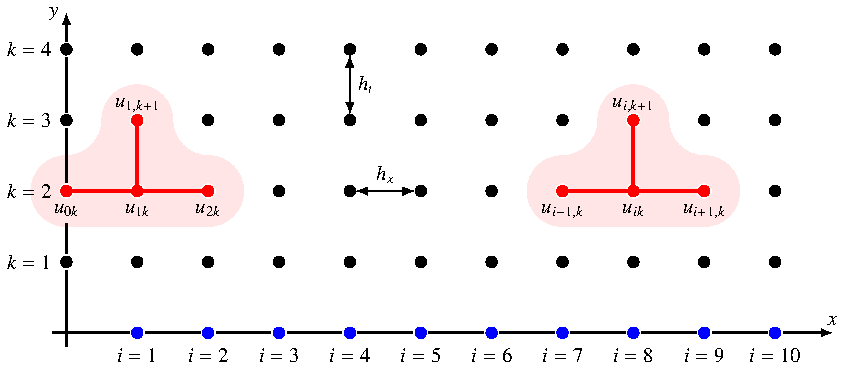
\includegraphics{chapters/70-pde/images/euler.pdf}
\caption{Euler-Verfahren für das Wärmeleitungsproblem.
\label{buch:pde:figure:euler}}
\end{figure}
Wir müssen jetzt die Differentialgleichung des Wärmelitungsproblems
diskretisieren.
Für die zweite Ableitung verwenden wir zweite Differenzen
Für die ersten Ableitungen haben wir verschiedene Optionen, wir
verwenden Vorwärtsdifferenzen, also
\begin{align}
\frac{\partial u}{\partial x}(x_{ik})
\simeq
\frac{u_{i,k+1}-u_{ik}}{h_t}
&=
\kappa
\frac{\partial^2u}{\partial x^2}(x_{ik})
\simeq
\kappa
\frac{u_{i,k-1}-2u_{ik}+u_{i,k+1}}{h_x^2}
\notag
\\
u_{i,k+1}
&=
u_{ik} + \frac{h_t\kappa}{h_x^2} (u_{i-1,k}-2u_{ik}+u_{i+1,k})
\label{buch:pde:waerme:euler}
\end{align}
für die inneren Punkte.
In Matrixform kann dies als
\[
\begin{pmatrix}
\vdots\\
u_{i,k+1}\\
\vdots
\end{pmatrix}
=
\begin{pmatrix}
&&&&\\
0&\dots
	&\displaystyle\frac{h_t\kappa}{h_x^2}
		&\displaystyle1-\frac{2h_t\kappa}{h_x^2}
			&\displaystyle\frac{h_t\kappa}{h_x^2}
				&\dots
					&0\\
&&&&
\end{pmatrix}
\begin{pmatrix}
\vdots\\
u_{i-1,k}\\
u_{ik}\\
u_{i+1,k}\\
\vdots
\end{pmatrix}
\]
geschrieben werden.
Wir kürzen den gemeinsamen Faktor $c=h_t\kappa/h_x^2$ ab und erhalten
die Form
\[
u_{k+1}
=
\begin{pmatrix}
\ddots&\ddots&\ddots&    &      &      &      \\
      &     c&  1-2c&  c &      &      &      \\
      &      &    c &1-2c&  c   &      &      \\
      &      &      &  c &1-2c  &  c   &      \\
      &      &      &    &\ddots&\ddots&\ddots
\end{pmatrix}
u_k.
\]
Die Lösung wird sich durch Iteration dieser Matrix finden lassen,
Konvergenz wird allein von $c$ abhängen.
Wir erwarten also, ein Konvergenz-Kriterium basierend auf $c$.

Die Gleichung~\eqref{buch:pde:waerme:euler} gilt nur für innere Punkte.
Für die Variablen $u_{0k}$, $u_{1k}$, $u_{N-1,k}$ und $u_{Nk}$ müssen
wir aus den Randbedingungen zusätzliche Gleichungen für die Randwerte
ableiten müssen.

\subsubsection{Rückwärts-Verfahren}
\begin{figure}
\centering
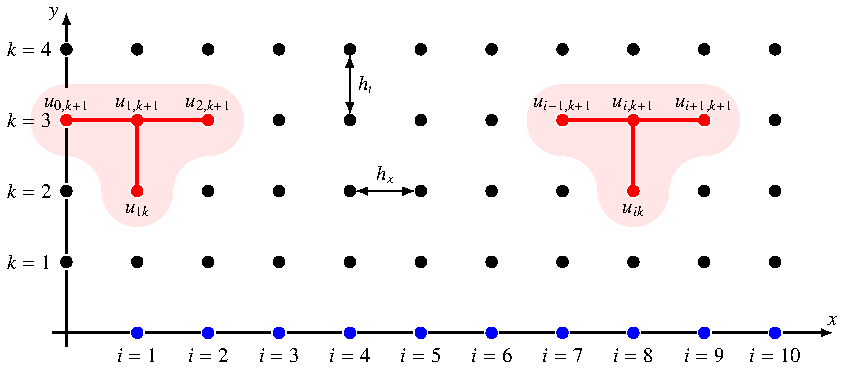
\includegraphics{chapters/70-pde/images/rueckwaerts.pdf}
\caption{Verwendung von Rückwärts-Differenzen für die Wärmeleitungsgleichung
\label{buch:pde:figure:rueckwaerts}}
\end{figure}
Statt der Vorwärts-Differenz kann man auch die Rückwärts-Differenz für
die erste Ableitung nach der Zeit verwenden.
Die diskretisierte Gleichung wird dann
\begin{align*}
\frac{u_{ik}-u_{i,k-1}}{h_t}
\simeq
\frac{\partial u}{\partial x}(x_{ik})
&=
\kappa\frac{\partial^2 u}{\partial x^2}(x_{ik})
\simeq
\frac{u_{i-1,k}-2u_{ik} + u_{i+1,k}}{h_x}.
\\
-cu_{i-1,k}
+
(1+2c)u_{ik}
-cu_{i+1,k}
&=u_{i,k-1}.
\end{align*}
In Matrixform kann man dies als
\[
\begin{pmatrix}
%\ddots&\ddots&\ddots&    &      &      &      \\
      &    -c&  1+2c& -c &      &      &      \\
      &      &   -c &1+2c& -c   &      &      \\
      &      &      & -c &1+2c  & -c   &      \\
      &      &      &    &\ddots&\ddots&\ddots
\end{pmatrix}
u_k
=
u_{k-1}
\]
schreiben.
Wieder gelten diese Gleichungen nur für innere Punkte.
Abbildung~\ref{buch:pde:figure:rueckwarts} zeigt, wie die Gleichungen
die Knotenwerte untereinander verknüpfen.

\subsubsection{Crank-Nicholson-Verfahren}
\begin{figure}
\centering
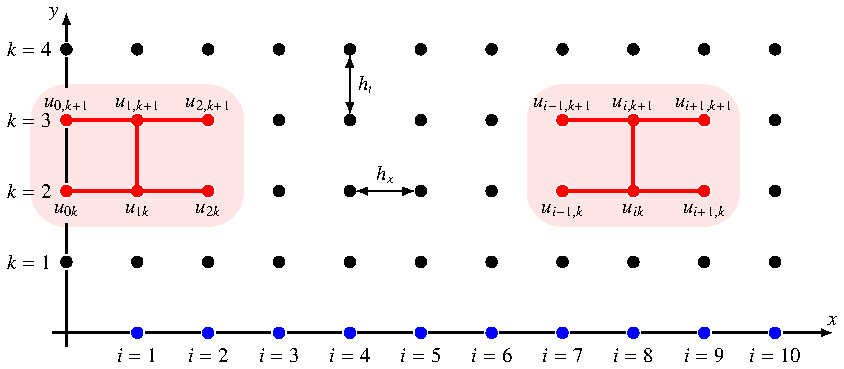
\includegraphics{chapters/70-pde/images/cngrid.pdf}
\caption{Verwendung der Knotenvariablen im Crank-Nicholson-Verfahren.
\label{buch:pde:figure:cngrid}}
\end{figure}
Sowohl Vorwärts- wie auch Rückwärts-Differenzen bestimmen die erste
Ableitung nach der Zeit eigentlich für einen Zeitpunkt zwischen 
den Vielfachen von $h_t$.
Für diese Zeitpunkte stehen aber keine Funktionswerte zur Verfügung, 
um damit die Gleichung aufzustellen.
Das Crank-Nicholson-Verfahren schlägt daher vor, den Mittelwert der
zweiten Ableitungen zu benachbarten Zeitpunkten als Wert für den
Zwischenzeitpunkt zu verwenden.
Damit wird die Wärmeleitungsgleichung approximiert durch
\begin{align*}
\frac{u_{i,k+1}-u_{ik}}{h_t}
\simeq
\frac{\partial u}{\partial x}(x_{ik})
&=
\kappa
\frac{\partial^2 u}{\partial x^2}(x_{ik})
\simeq
\frac{\kappa}2\biggl(
\frac{u_{i-1,k+1}-2u_{i,k+1}+u_{i+1,k+1}}{h_x^2}
+
\frac{u_{i-1,k}-2u_{i,k}+u_{i+1,k}}{h_x^2}
\biggr)
\\
2u_{i,k+1}-2u_{ik}
&=
c(
u_{i-1,k+1}-2u_{i,k+1}+u_{i+1,k+1}
+
u_{i-1,k}-2u_{i,k}+u_{i+1,k}
)
\end{align*}
Verschiebt man die Terme nach Zeitpunkt auf die beiden Seiten
der Gleichung erhält man
\begin{equation}
-cu_{i-1,k+1}+2(1+c)u_{i,k+1}-cu_{i+1,k+1}
=
cu_{i-1,k}+2(1-c)u_{i,k}+cu_{i+1,k},
\end{equation}
was sich leichter in Matrixform 
\begin{equation}
\begin{pmatrix}
&\ddots& \ddots &        &        &        &        \\
&  -c  & 2(1+c) &  -c    &        &        &        \\
&      &  -c    & 2(1+c) &  -c    &        &        \\
&      &        &  -c    & 2(1+c) &  -c    &        \\
&      &        &        & \ddots & \ddots &        
\end{pmatrix}
u_{k+1}
=
\begin{pmatrix}
&\ddots&\ddots  &        &        &        &        \\
&   c  & 2(1-c) &   c    &        &        &        \\
&      &   c    & 2(1-c) &   c    &        &        \\
&      &        &   c    & 2(1-c) &   c    &        \\
&      &        &        &\ddots  & \ddots &        
\end{pmatrix}
u_k
\end{equation}
bringen lässt.

\subsection{Wärmeleitungsgleichung mit Dirichlet-Randbedingungen
\label{buch:pde:subsection:waerme:dirichlet}}
Die bisher formulierten Gleichungen berücksichtigen die
Randbedingungen nicht.
Dirichlet-Rand\-bedingungen am linken und rechten Rand des Intervalls
legen die Werte $u_{0k}$ und $u_{Nk}$ fest.
Wir möchten dies wieder in Matrixform schreiben.
Da die Randbedingungen nicht von $u$ abhängen, muss dies in der Form
$u_{k+1}=Au_k + b_k$ möglich sein, was nur geht, wenn
\begin{equation}
u_{k+1}
=
\underbrace{
\begin{pmatrix}
 0  &   0  &  0   &      &      &      &      &      &      \\
 c  & 1-2c &  c   &      &      &      &      &      &      \\
    &  c   & 1-2c &  c   &      &      &      &      &      \\
    &      &\ddots&\ddots&\ddots&      &      &      &      \\
    &      &      &  c   & 1-2c &  c   &      &      &      \\
    &      &      &      &\ddots&\ddots&\ddots&      &      \\
    &      &      &      &      &  c   & 1-2c &  c   &      \\
    &      &      &      &      &      &  c   & 1-2c &  c   \\
    &      &      &      &      &      &  0   &  0   &  0   
\end{pmatrix}}_{\displaystyle A\mathstrut}
u_k
+
\underbrace{
\begin{pmatrix}
g_{0k}\\
0     \\
0     \\
\vdots\\
0     \\
\vdots\\
0     \\
0     \\
g_{Nk}
\end{pmatrix}}_{\displaystyle b_k\mathstrut}
\end{equation}
für die Randwerte $g$.

Für homogene Randbedingungen wird die Situation etwas einfacher zu
analysieren, denn dann ist $b_k=0$.
Wir erwarten, dass die Lösung exponentiell gegen $0$ konvergiert,
das System ``kühlt aus''.
Da die Randbedingungen $u_{0k}=u_{Nk}=0$ erzwingen, kann man diese 
Variablen weglassen die Vektoren $u$ und die Matrix $A$ verkürzen auf
\begin{equation}
\tilde{u}_{k+1}
=
\begin{pmatrix}
u_{1,k+1}\\
u_{2,k+1}\\
\vdots\\
u_{i,k+1}\\
\vdots\\
u_{N-1,k+1}\\
u_{N,k+1}
\end{pmatrix}
=
\underbrace{
\begin{pmatrix}
 1-2c &  c   &      &      &      &      &      \\
  c   & 1-2c &  c   &      &      &      &      \\
      &\ddots&\ddots&\ddots&      &      &      \\
      &      &  c   & 1-2c &  c   &      &      \\
      &      &      &\ddots&\ddots&\ddots&      \\
      &      &      &      &  c   & 1-2c &  c   \\
      &      &      &      &      &  c   & 1-2c \\
\end{pmatrix}}_{\displaystyle \tilde{A}\mathstrut}
\begin{pmatrix}
u_{1k}\\
u_{2k}\\
\vdots\\
u_{ik}\\
\vdots\\
u_{N-1,k}\\
u_{Nk}
\end{pmatrix}
=
A
\tilde{u}_k
\end{equation}
Die Lösung $u$ entsteht also durch Iteration mit der Matrix $\tilde{A}$.
Der Spektralradius der Matrix gibt Auskunft darüber, ob das Verfahren
konvergiert.
Da die Matrix $\tilde{A}$ symmetrisch ist, sind alle Eigenwerte reell.
\begin{figure}
\centering
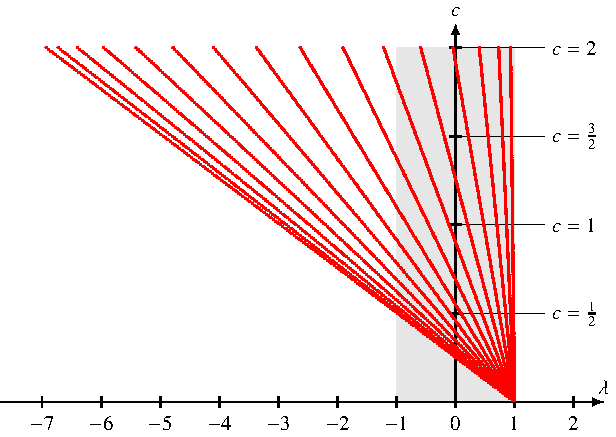
\includegraphics{chapters/70-pde/images/explizitspektrum.pdf}
\caption{Spektrum der Matrix $\tilde{A}$ für $N=16$,
die sich für das Euler-Verfahren mit
homogenen Dirichlet-Randwerte ergibt.
Nur für $c<2$ ist der Spektralradius $<1$.
\label{buch:pde:waerme:explizitspektrum}}
\end{figure}
In Abbildung~\ref{buch:pde:waerme:explizitspektrum} sind die Eigenwerte
von $\tilde{A}$ dargestellt.
Man kann erkennen, dass nur für $c<\frac12$ der Spektralradius $<1$
wird.
Daraus ergibt sich das Kriterium
\[
\frac{2\kappa h_t}{h_x^2} < 1
\]
für die Konvergenz des Verfahrens.

Für das Rückwärtsverfahren sieht die Matrix etwas anders aus, es gilt
\begin{equation}
\begin{pmatrix}
   0  &    0  &   0  &      &      &      &      &      &      \\
  -c  &  1+2c &  -c  &      &      &      &      &      &      \\
      &   -c  & 1+2c &  -c  &      &      &      &      &      \\
      &       &\ddots&\ddots&\ddots&      &      &      &      \\
      &       &      &  -c  & 1+2c &  -c  &      &      &      \\
      &       &      &      &\ddots&\ddots&\ddots&      &      \\
      &       &      &      &      &  -c  & 1+2c &  -c  &      \\
      &       &      &      &      &      &  -c  & 1+2c &  -c  \\
      &       &      &      &      &      &   0  &   0  &   0  
\end{pmatrix}
u_{k+1}
=
Bu_{k+1}
=
u_k + b_k
\end{equation}
Für den Fall homogener Randbedingungen werden auch hier wieder
nur die ``inneren'' Koeffizienten
\[
\tilde{B}
=
\begin{pmatrix}
 1+2c &  -c  &      &      &      &      &      \\
  -c  & 1+2c &  -c  &      &      &      &      \\
      &\ddots&\ddots&\ddots&      &      &      \\
      &      &  -c  & 1+2c &  -c  &      &      \\
      &      &      &\ddots&\ddots&\ddots&      \\
      &      &      &      &  -c  & 1+2c &  -c  \\
      &      &      &      &      &  -c  & 1+2c 
\end{pmatrix}
\]
der Matrix $B$ nötig.
Die Lösung findet man dann aus $\tilde{B}\tilde{u}_{k+1}=\tilde{u}_k$
durch Iteration $\tilde{u}_{k+1}=\tilde{B}^{-1} \tilde{u}_k$.
Konvergenz wird wieder bestimmt durch den Spektralradius $\varrho{\tilde{B}}$,
der, wie Abbildung~\ref{buch:pde:waerme:implizitspektrum} zeigt, immer
$<1$ ist.
Das Rückwärtsverfahren ist also immer konvergent, ganz unabhängig von
den relativen Schrittweiten.
\begin{figure}
\centering
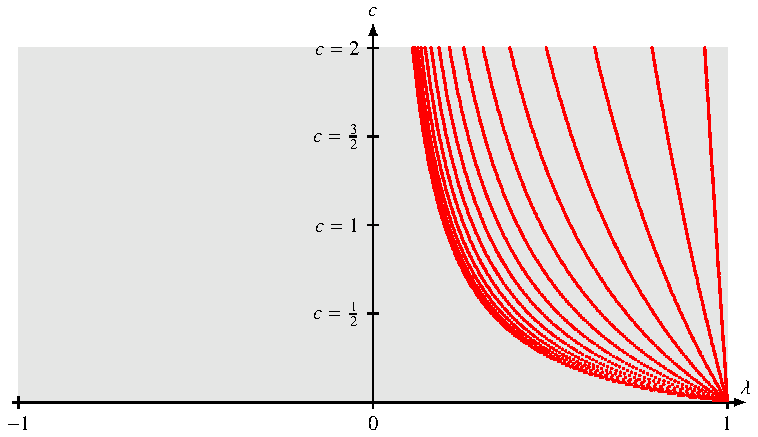
\includegraphics{chapters/70-pde/images/implizitspektrum.pdf}
\caption{Eigenwertspektrum der Matrix $\tilde{B}^{-1}$ für das 
Rückwärts-Verfahren.
Der Spektralradius ist unabhängig von $c$ immer $<1$.
\label{buch:pde:waerme:implizitspektrum}}
\end{figure}

Für das Crank-Nicholson-Verfahren ist, welches wir hier nur für homogene
Randbedingungen betrachten wollen.
Aus der Gleichung
\begin{gather*}
\tilde{C}u_{k+1}
=
\begin{pmatrix}
2(1+c)&  -c  &      &      &      &      &      \\
   -c &2(1+c)&  -c  &      &      &      &      \\
      &   -c &2(1+c)&  -c  &      &      &      \\
      &      &\ddots&\ddots&\ddots&      &      \\
      &      &      &\ddots&\ddots&\ddots&      \\
      &      &      &      &   -c &2(1+c)&  -c  \\
      &      &      &      &      &  -c  &2(1+c)
\end{pmatrix}
u_{k+1}
\qquad
\qquad
\qquad
\\
\qquad
\qquad
\qquad
=
\tilde{D}u_{k}
=
\begin{pmatrix}
2(1-c)&   c  &      &      &      &      &      \\
    c &2(1-c)&   c  &      &      &      &      \\
      &    c &2(1-c)&   c  &      &      &      \\
      &      &\ddots&\ddots&\ddots&      &      \\
      &      &      &\ddots&\ddots&\ddots&      \\
      &      &      &      &    c &2(1-c)&   c  \\
      &      &      &      &      &   c  &2(1-c)
\end{pmatrix}
u_k
\end{gather*}
folgern wir, dass die Iteration $u_{k+1} = \tilde{C}^{-1}\tilde{D} u_k$
die Lösung der Gleichung liefert.
\begin{figure}
\centering
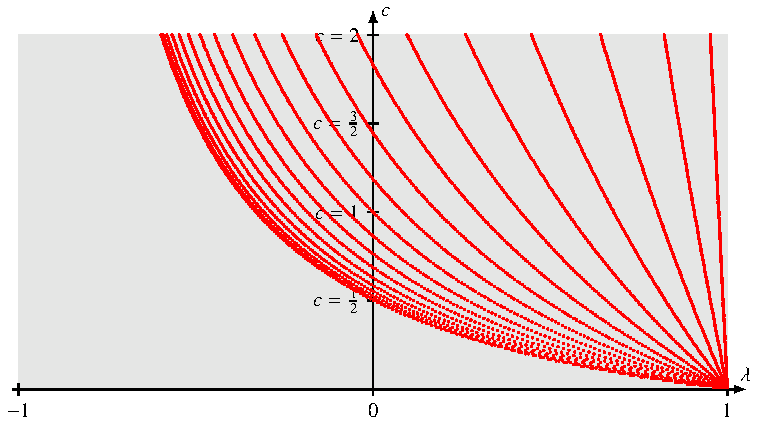
\includegraphics{chapters/70-pde/images/cnspektrum.pdf}
\caption{Eigenwertspektrum für das Crank-Nicholson-Verfahren
\label{buch:pde:waerme:cnspektrum}}
\end{figure}
Das Spektrum von $\tilde{C}^{-1}\tilde{D}$ ist in
Abbildung~\ref{buch:pde:waerme:cnspektrum} dargestellt und zeigt,
dass auch das Crank-Nicholson-Verfahren immer konvergiert unabhängig von
der Schrittweite $h_t$.

\subsection{Wärmeleitungsgleichung mit Neumann-Randbedingungen
\label{buch:pde:subsection:waerme:neumann}}
Die Neumann-Randbedingungen legen nicht Werte in den Randpunkten fest,
sondern liefern nur Gleichungen zwischen den Variablen nahe dem Rand.
Sie ändern damit die Koeffizientenmatrix des Gleichungssystems und haben
nicht nur Einfluss auf konstante Vektoren $b_k$ wie in
Abschnitt~\ref{buch:pde:subsection:waerme:dirichlet}.

\subsubsection{Neumann-Randbedingungen}
Wir betrachten in diesem Abschnitt nur homogene Neumann-Randbedingungen.
Die Randbedingung am linken und rechten Rand verlangt, dass $u_{0k}=u_{1k}$
und $u_{N-1,k}=u_{Nk}$ gelten muss.
Dies bedeutet, dass die Randwerte $u_{0k}$ und $u_{Nk}$ mit der
gleichen Formel berechnet werden können wie die Werte für $u_{1k}$ und
$u_{N-1,k}$.
Wir können damit die Variablen $u_{0k}$ und $u_{Nk}$ aus allen
Gleichungen eliminieren, indem wir sie durch $u_{1k}$ und $u_{N-1,k}$ 
ersetzen.

\subsubsection{Euler-Verfahren}
Aus den Gleichungen
\begin{align*}
u_{1,k+1} &= c u_{0k} + (1-2c) u_{1k} + c u_{2k} \\
u_{N-1,k+1} &= c u_{N-2,k} + (1-2c) u_{N-1,k} + c u_{Nk} 
\end{align*}
am Rand des Gebietes werden nach den Ersetzungen
$u_{0k}\to u_{1k}$
und
$u_{Nk}\to u_{N-1,k}$
die Gleichungen
\begin{align*}
u_{1,k+1}
&=
(1-c) u_{1k} + c u_{2k}
\\
u_{N-1,k+1}
&=
c u_{N-2,k} + (1-c) u_{N-1,k}.
\end{align*}
Die Matrix des Euler-Verfahrens wird damit zu
\begin{equation}
\tilde{u}_{k+1}
=
\underbrace{
\begin{pmatrix}
 1- c &  c   &      &      &      &      &      \\
  c   & 1-2c &  c   &      &      &      &      \\
      &\ddots&\ddots&\ddots&      &      &      \\
      &      &  c   & 1-2c &  c   &      &      \\
      &      &      &\ddots&\ddots&\ddots&      \\
      &      &      &      &  c   & 1-2c &  c   \\
      &      &      &      &      &  c   & 1- c 
\end{pmatrix}}_{\displaystyle A}
\tilde{u}_k.
\end{equation}
Die Konvergenz des Verfahrens hängt wieder vom Spektralradius ab.
Diesmal können wir aber nicht erwarten, dass alle Eigenwerte
Betrag $<1$ haben werden.
Die Zeilen- und Spaltensumme der Matrix $A$ ist immer $1$, d.~h.~die
ein konstanter Vektor wird auf sich selbst abgebildet.
Insbesondere gibt es einen Eigenvektor zum Eigenwert $1$,
der Spektralradius kann also nicht kleiner als $1$ sein. 
\begin{figure}
\centering
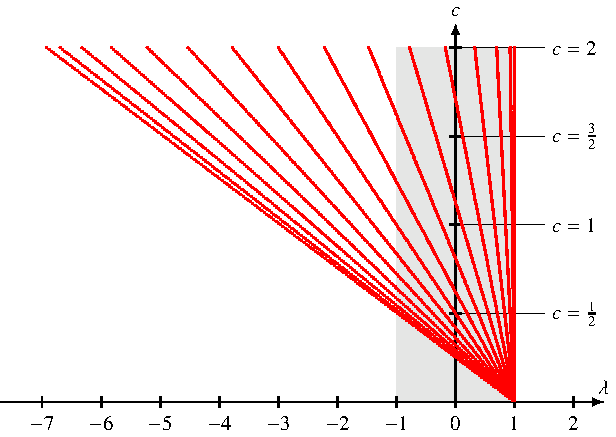
\includegraphics{chapters/70-pde/images/explizitneumann.pdf}
\caption{Eigenwertspektrum des Euler-Verfahrens für
Neumann-Randbedingungen.
Der Eigenwert $1$ ist einfach,
für $c<\frac12$ ist der Spektralradius $1$.
\label{buch:pde:waerme:explizit:neumannspektrum}}
\end{figure}
Für $c<1$ konvergiert das Verfahren daher gegen die konstante
Temperaturverteilung.
\begin{figure}
\centering
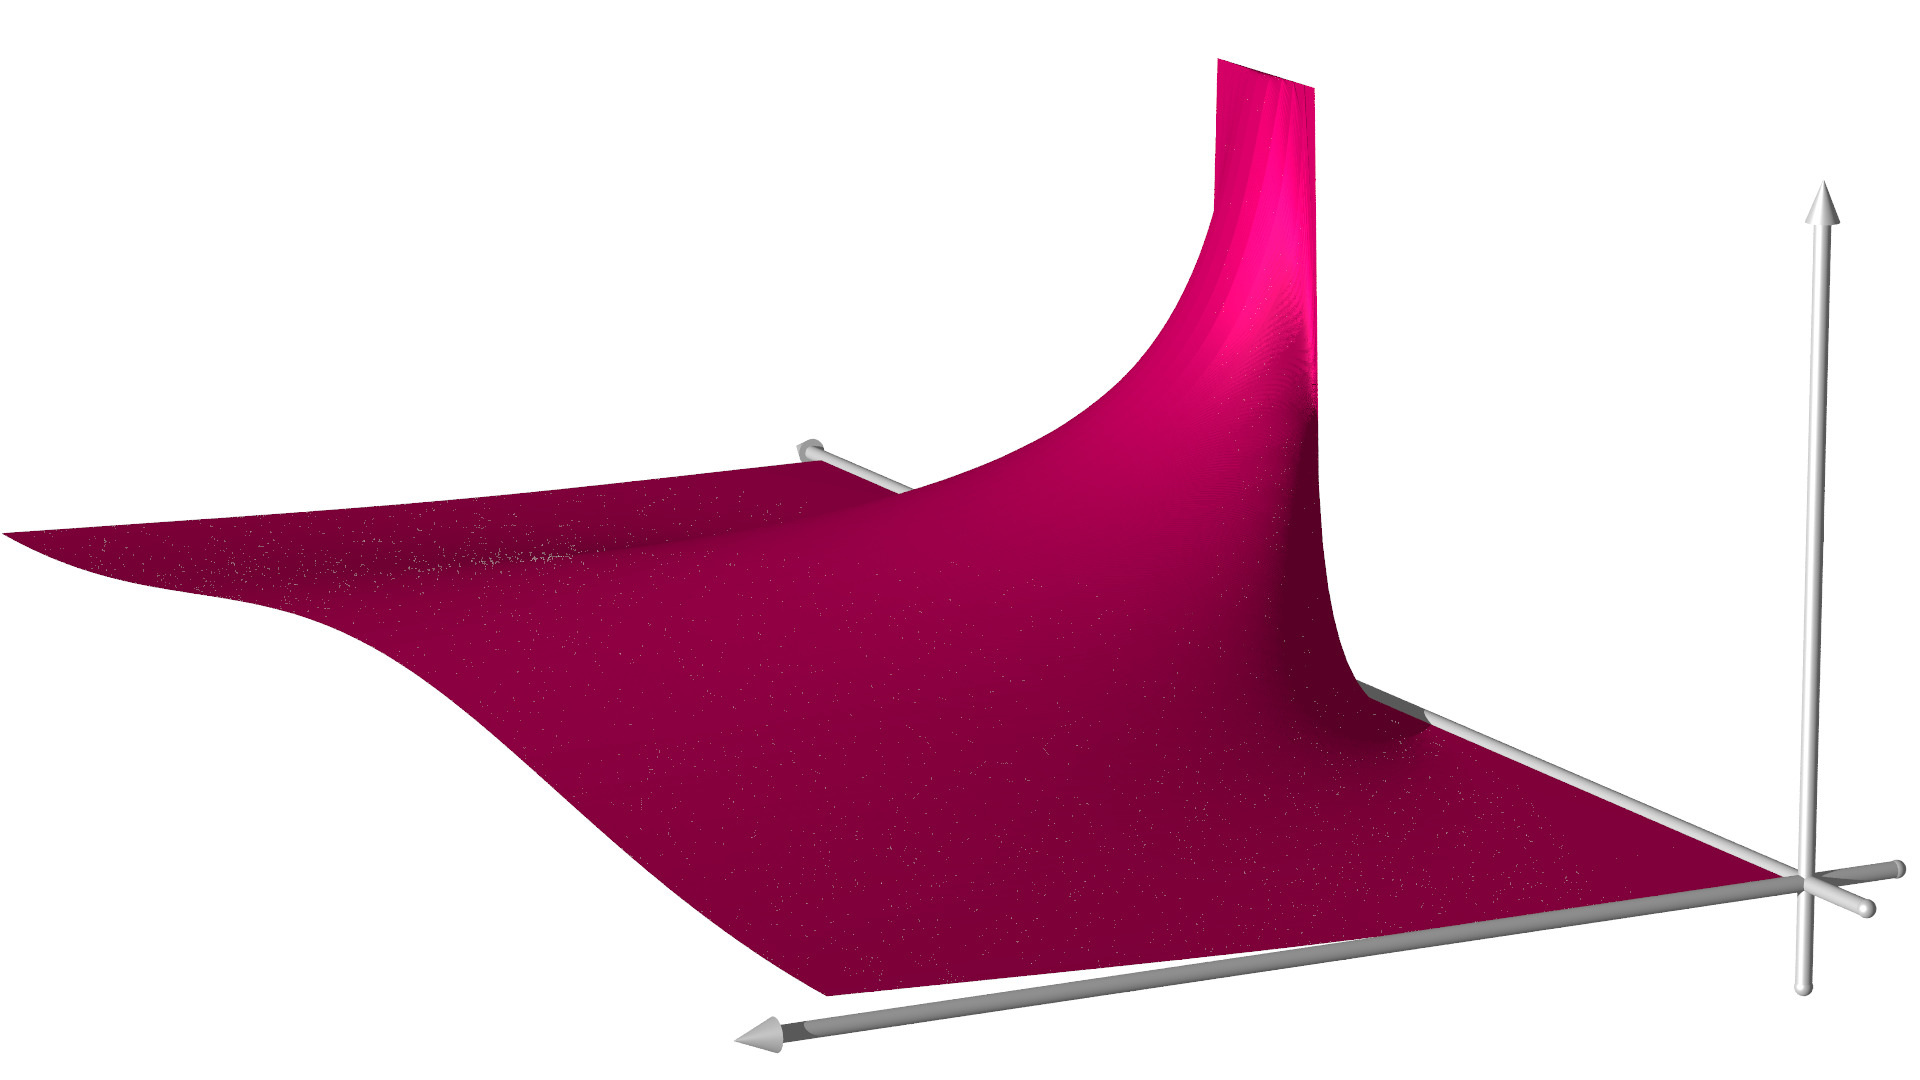
\includegraphics[width=\hsize]{chapters/70-pde/images/explizit.jpg}
\caption{Lösung der Wärmeleitungsgleichung mit dem Eulerverfahren.
\label{buch:pde:waerme:figure:euler}}
\end{figure}
Die numerische Durchführung des Verfahrens mit geeigneten Werten von
$h_x$ und $h_t$ derart, dass $c<\frac12$ ist, führt auf die
Lösungsfläche in Abbildung~\ref{buch:pde:waerme:figure:euler}.

\subsubsection{Rückwärtsverfahren}
Auch für das Rückwärtsverfahren können wir für Neumann-Randbedinungen
die Matrixgleichung
\begin{equation}
Bu_k
=
\begin{pmatrix}
 1+c & -c   &      &      &      &      &      &     \\
 -c  & 1+2c & -c   &      &      &      &      &     \\
     &  -c  & 1+2c & -c   &      &      &      &     \\
     &      &\ddots&\ddots&\ddots&      &      &     \\
     &      &      &\ddots&\ddots&\ddots&      &     \\
     &      &      &      &  -c  & 1+2c & -c   &     \\
     &      &      &      &      &  -c  & 1+2c & -c  \\
     &      &      &      &      &      &  -c  & 1+c 
\end{pmatrix}
u_k
=
u_{k-1}
\end{equation}
finden.
Auch diese Matrix hat den konstanten Vektor als einzigen Eigenvektor
zum Eigenwert $1$.
Wie bei Dirichlet-Randbedingungen ist das Spektrum, dargestellt in
Abbildung~\ref{buch:pde:waerme:implizit:neumannspektrum}, bis auf den
einen Eigenwert $1$ im Intervall $(0,1)$ enthalten, so dass das
Verfahren konvergiert.
Die Lösung ist dargestellt in
Abbildung~\ref{buch:pde:waerme:figure:rueckwaerts}.
\begin{figure}
\centering
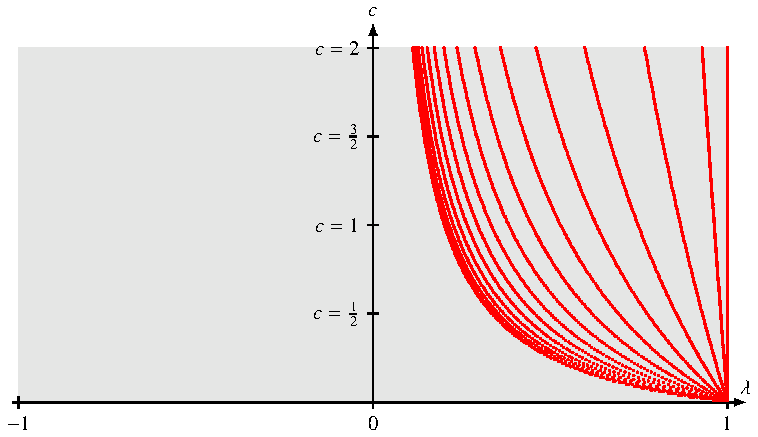
\includegraphics{chapters/70-pde/images/implizitneumann.pdf}
\caption{Das Eigenwertspektrum für das Rückwärtsverfahren für
Neumann-Randbedingungen enthält eine einzelnen Eigenwert $1$, alle
anderen Eigenwerte haben Betrag $<1$.
\label{buch:pde:waerme:implizit:neumannspektrum}}
\end{figure}
\begin{figure}
\centering
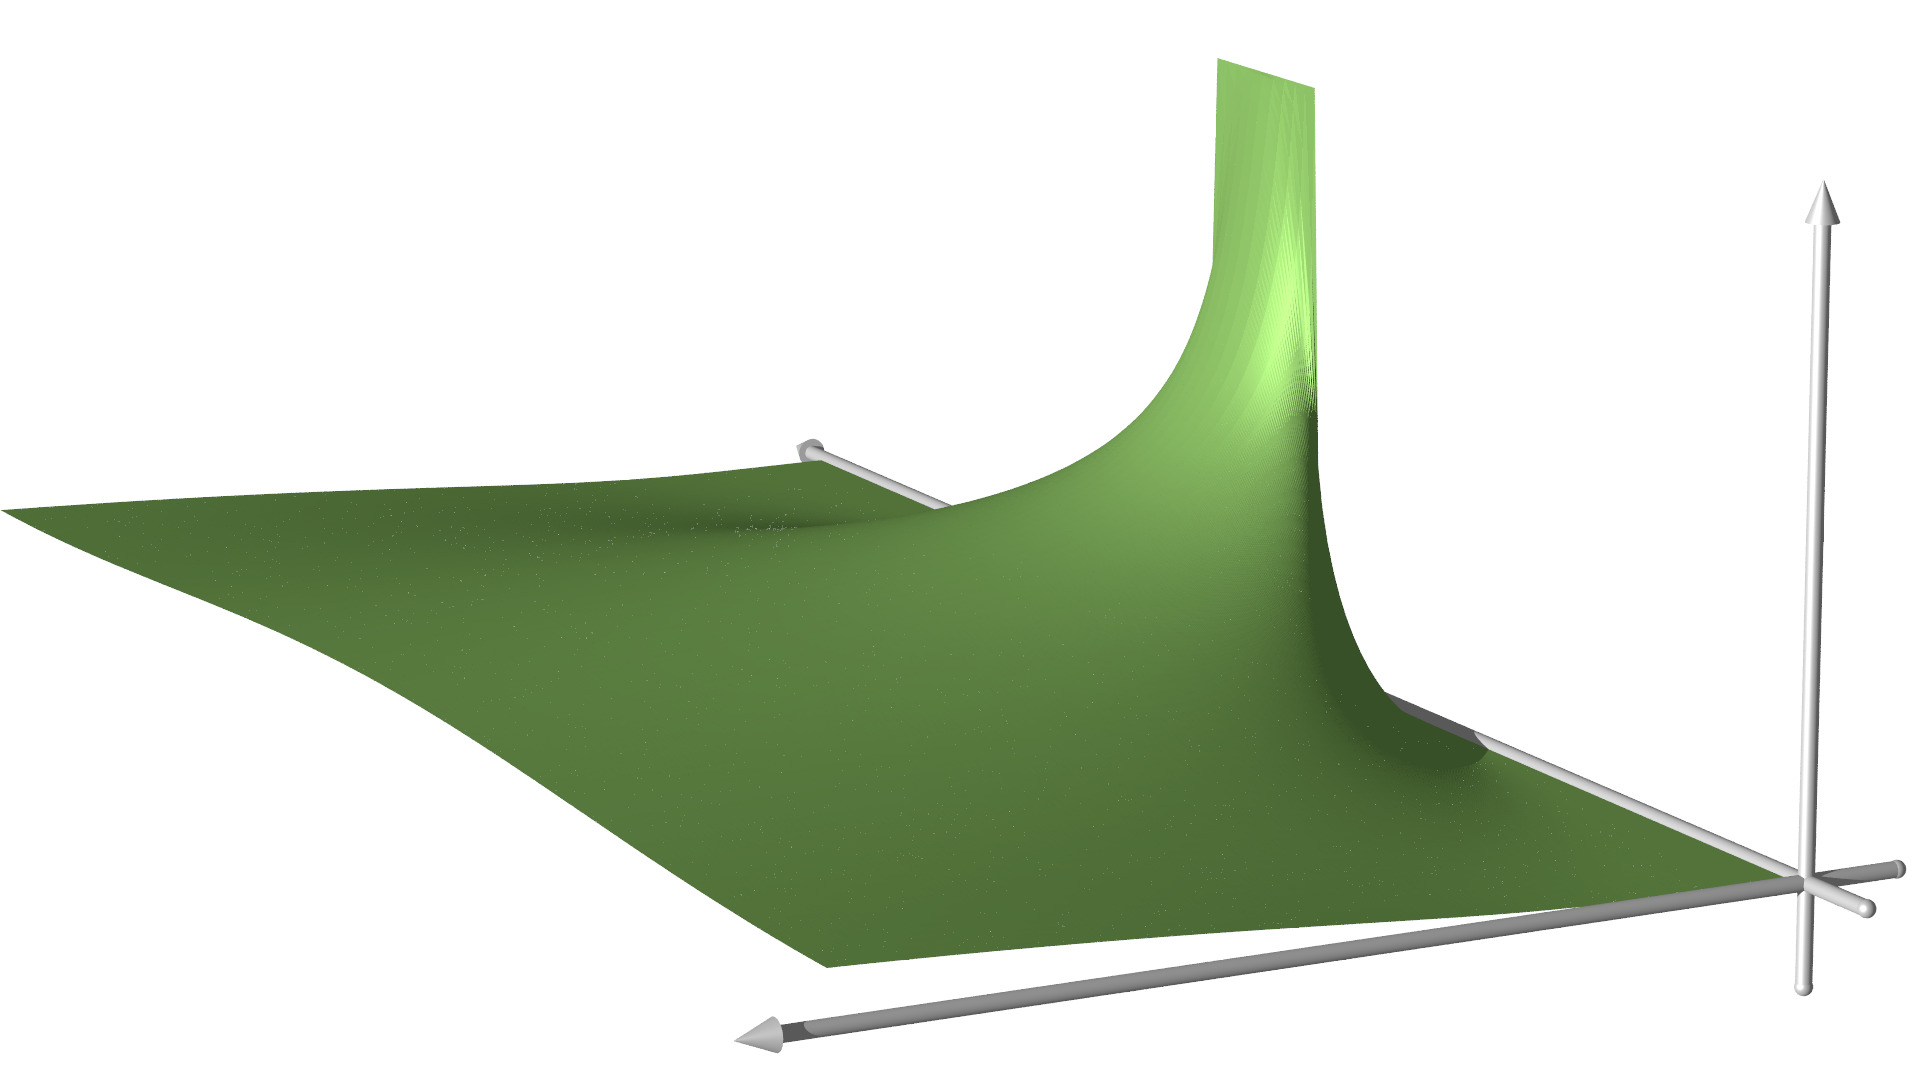
\includegraphics[width=\hsize]{chapters/70-pde/images/implizit.jpg}
\caption{Lösung der Wärmeleitungsgleichung mit dem Rückwärtsverfahren.
\label{buch:pde:waerme:figure:rueckwaerts}}
\end{figure}

\subsubsection{Crank-Nicholson-Verfahren}
Für das Crank-Nicholson-Verfahren sind die Gleichungen am Rand
des Intervals
\begin{align*}
-cu_{0,k+1}+2(1+c)u_{1,k+1}-cu_{2,k+1}
&=
cu_{0k}+2(1-c)u_{1k}+cu_{2,k}
\\
(2+c)u_{1,k+1}-cu_{2,k+1}
&=
(2-c)u_{1k}+cu_{2,k},
\end{align*}
so dass die Matrixgleichung
\begin{gather*}
Cu_{k+1}
=
\begin{pmatrix}
 2+c &  -c  &      &      &      &      &      \\
  -c &2(1+c)&  -c  &      &      &      &      \\
     &   -c &2(1+c)&  -c  &      &      &      \\
     &      &\ddots&\ddots&\ddots&      &      \\
     &      &      &\ddots&\ddots&\ddots&      \\
     &      &      &      &   -c &2(1+c)&  -c  \\
     &      &      &      &      &  -c  &  2+c
\end{pmatrix}
u_{k+1}
\qquad
\qquad
\qquad
\\
\qquad
\qquad
\qquad
=
\begin{pmatrix}
 2-c &   c  &      &      &      &      &      \\
   c &2(1-c)&   c  &      &      &      &      \\
     &    c &2(1-c)&   c  &      &      &      \\
     &      &\ddots&\ddots&\ddots&      &      \\
     &      &      &\ddots&\ddots&\ddots&      \\
     &      &      &      &    c &2(1-c)&   c  \\
     &      &      &      &      &   c  &  2-c
\end{pmatrix}
u_k
=
Du_k
\end{gather*}
wird.
Daraus erhält man als Iterationsverfahren:
\[
u_{k+1} = C^{-1}Du_k.
\]
Das Eigenwertspektrum (Abbildung~\ref{buch:pde:waerme:cranknicholson:spektrum})
hat wieder einen einfachen Eigenwert $1$,
alle anderen Eigenwerte haben Betrag $<1$, das Verfahren ist
konvergent obwohl der Spektralradius exakt $1$ ist.
\begin{figure}
\centering
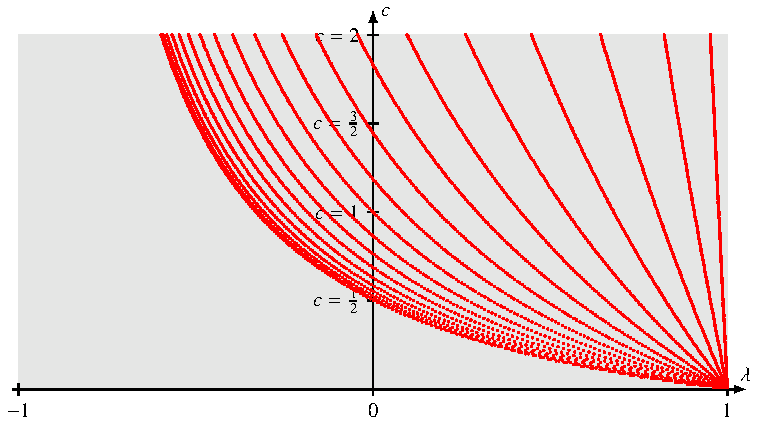
\includegraphics{chapters/70-pde/images/cnspektrum.pdf}
\caption{Das Eigenwertspektrum des Crank-Nicholson-Verfahrens zeigt
einen einzelnen Eigenwert $1$ 
\label{buch:pde:waerme:cranknicholson:spektrum}}
\end{figure}
\begin{figure}
\centering
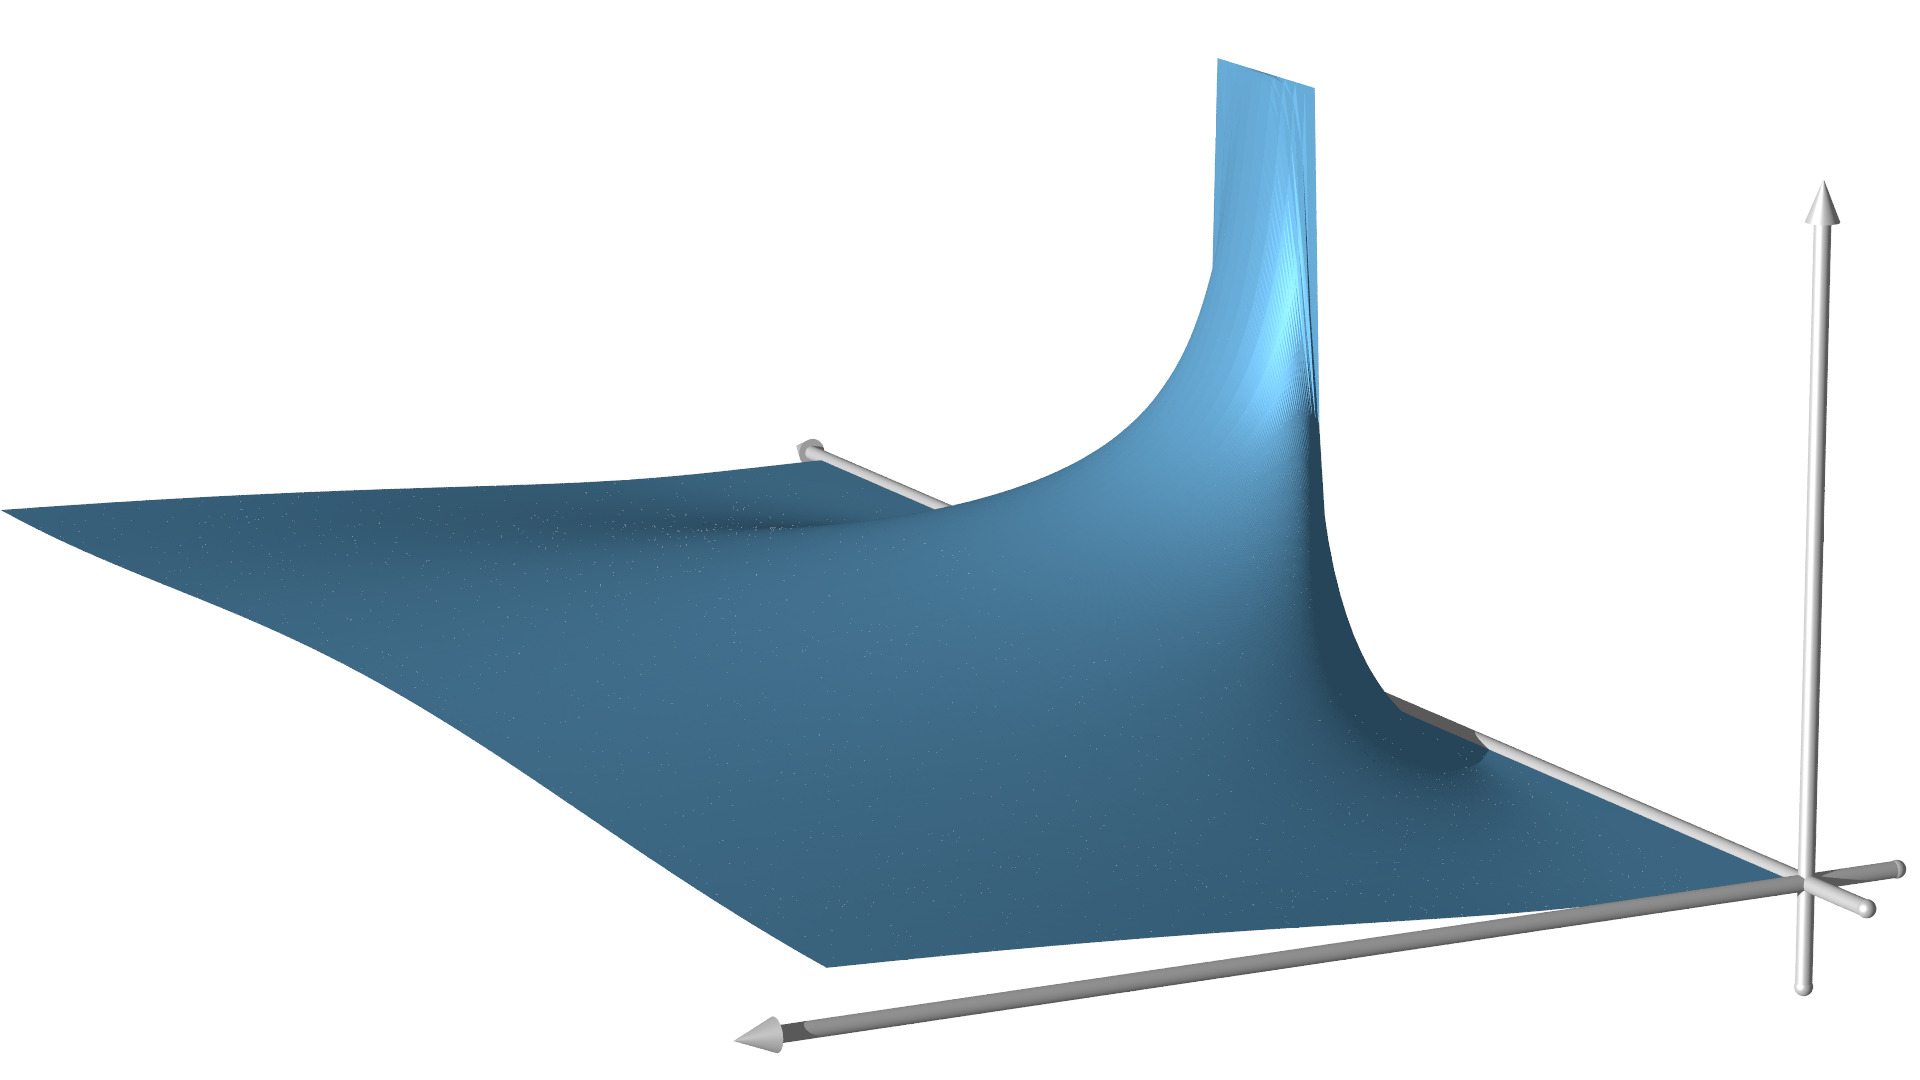
\includegraphics[width=\hsize]{chapters/70-pde/images/cranknicholson.jpg}
\caption{Lösung der Wärmeleitungsgleichung mit dem Crank-Nicholson-Verfahren
\label{buch:pde:waerme:figure:cranknicholson}}
\end{figure}

\begin{figure}
\centering
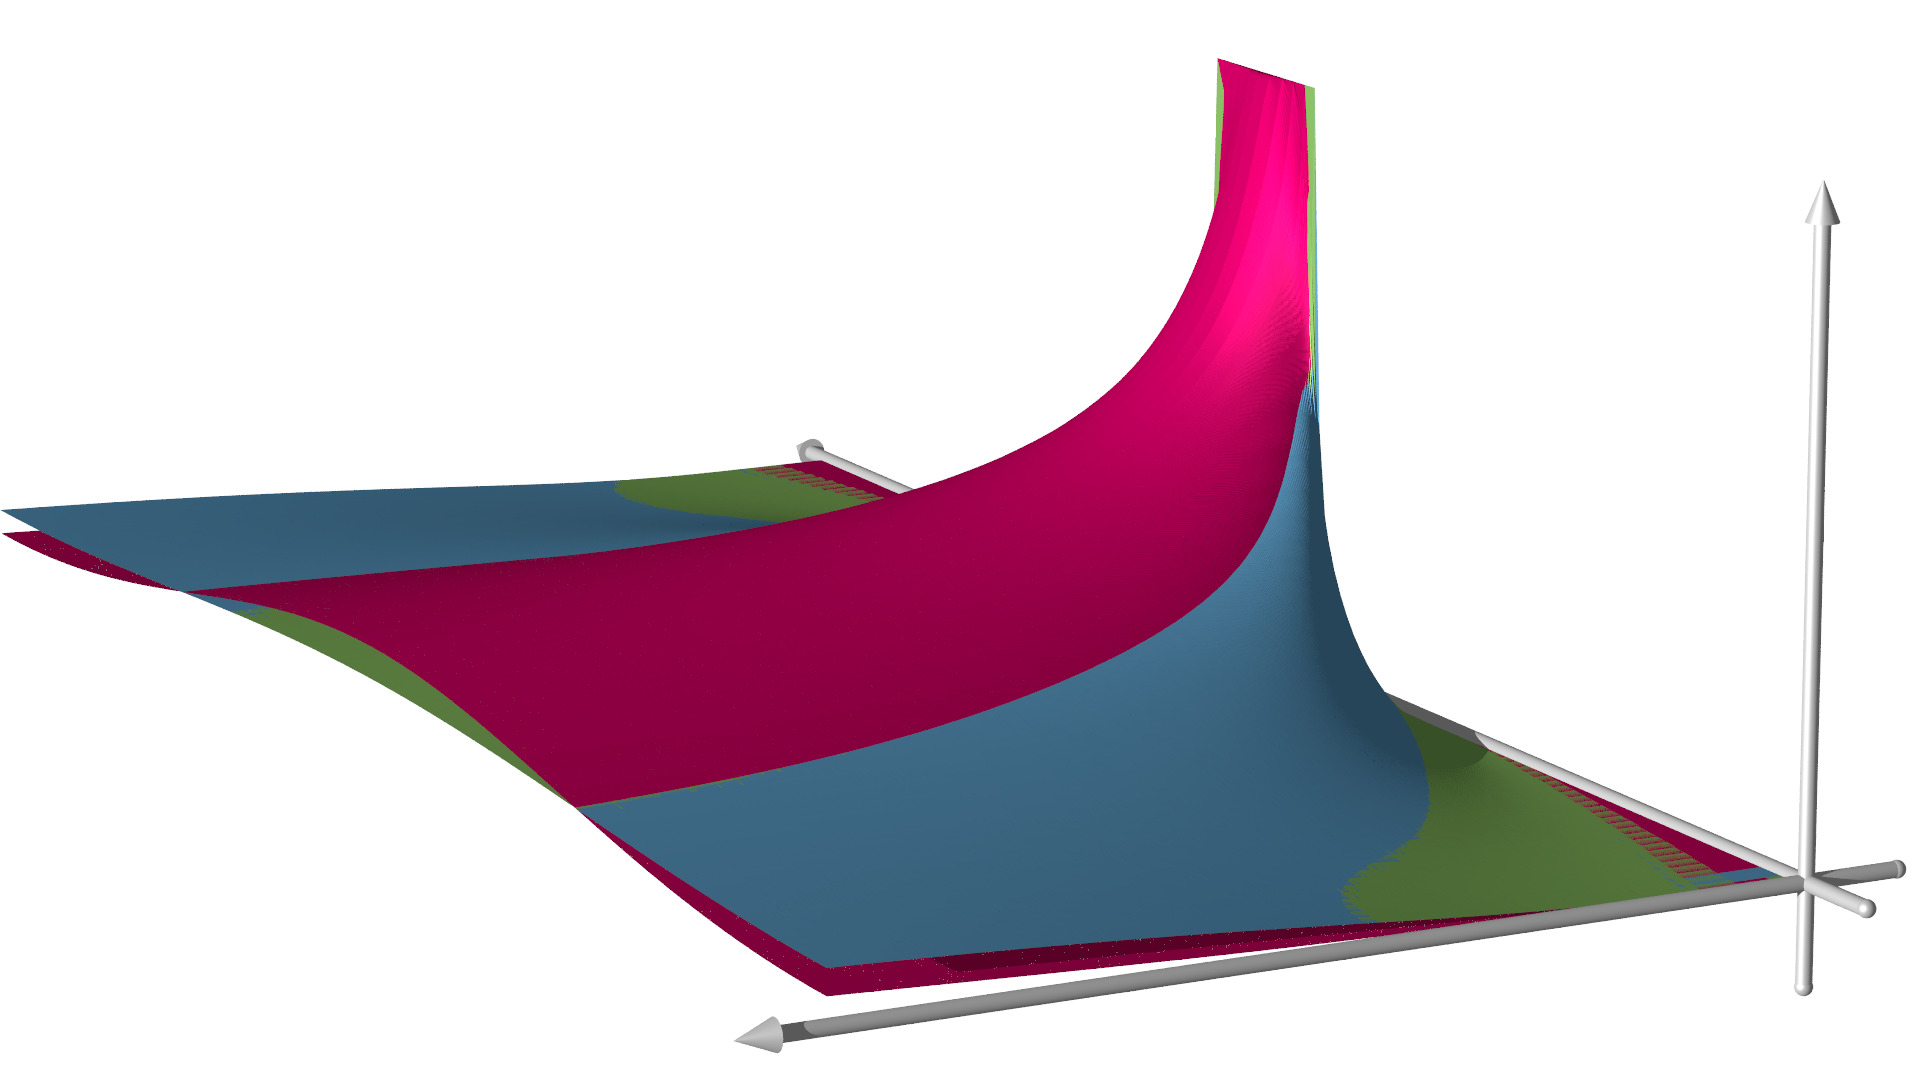
\includegraphics[width=\hsize]{chapters/70-pde/images/combined.jpg}
\caption{Alle drei Lösungsverfahren liefern ähnliche Lösungen,
doch das Euler-Verfahren (rot) weicht stark von den beiden anderen
Verfahren ab.
Das Rückwärts-Verfahren und das Crank-Nicholson-Verfahren stimmen
weitgehend überein.
\label{buch:pde:waerme:figure:combined}}
\end{figure}
In Abbildung~\ref{buch:pde:waerme:figure:combined} sind die drei
Lösungen im gleichen Graphen dargestellt. 
Die Lösung des Euler-Verfahrens weicht stark von den anderen Verfahren ab.
Die Wärmeleitungsgleichung hat Lösungen, bei denen sich Wärme mit
unendlicher Geschwindigkeit ausbreitet.
Im Euler-Verfahren kann sich ein Temperatursprung nur um $h_x$ in
jeder Iteration ausbreiten, also maximal mit der Geschwindigkeit $h_x/h_t$.
Daher verhält sich das Euler-Verfahren so, wie wenn die Wärmeleitfähigkeit
reduziert wäre, was zu dem ausgeprägteren Buckel der Euler-Lösung
führt.


